\clearpage

\section{IP Tunnel MS Windows}

\begin{tcolorbox}	
	\begin{tabular}{p{2.75cm} p{0.2cm} p{10.5cm}} 	
		\textbf{Header File}   &:& ip$\_$tunnel$\_$ms$\_$windows$\_*$.h \\
		\textbf{Source File}   &:& ip$\_$tunnel$\_$ms$\_$windows$\_*$.cpp \\
        \textbf{Version}       &:& 20180815 (Jo\~ao Coelho) \\
	\end{tabular}
\end{tcolorbox}

This block works in two ways: one way with one input and zero output signals (as client/sender) and the other one with zero input and one output signal (as server/receiver).
IP Tunnel MS Windows is duplicated onto two machines; the first takes samples out of the input buffer until it's empty and transmits them to the IP Tunnel on the second machine through a TCP/IP connection. The IP Tunnel on the second machine receives the signal and outputs it to the output buffer.
It's only necessary to specify the ip address of the remote machine and its TCP port. \par
After some tests on the computer lab, from a total of 100 Mbps of bandwith on the ethernet port, the average bandwith used on the simulation is 73 Mbps (around 73\%). 
\par
Currently, the IP Tunnel works between two machines on the same network or within the same VPN setup.
To work between two different networks without a VPN setup, a TCP Nat Traversal/Hole Punching structure would have to be implemented. This consists in a new module, that works as a intermediary between the client and the server. These, connect to the mediator (getting their IP addresses), following with the transmission of each other's addresses and its connection.
\par
Only works on windows due to the Ws2tcpip.h header and ws2\_32 library and it is compatible and tested with SDK v8.1 and v10.0.18362.0.

\subsection*{Input Parameters}

\begin{table}[h]
	\centering
	\begin{tabular}{|l|c|c|c|p{50mm}|}
		\cline{1-5}
		\textbf{Parameter} & \textbf{Type} & \textbf{Values} &   \textbf{Default}& \textbf{Brief Description} \\ \cline{1-5}
		
        displayNumberOfSamples & bool & true/false & true & If true, number of samples sent and received are displayed.\\ \cline{1-5}
		numberOfTrials & int & any & $10$ & Number of trials after a connection has been refused.\\ \cline{1-5}
		remoteMachineIpAddress & string & any & "127.0.0.1" & IP Address of Remote Machine.\\ \cline{1-5}
		tcpPort & int & any & $54000$ & TCP port used to connect to server.\\ \cline{1-5}
		timeIntervalSeconds & int & any & $3$ & Time interval before trying to connect again after a connection has been refused (seconds).\\ \cline{1-5}
	\end{tabular}
	\caption{IP Tunnel MS Windows input parameters}
	\label{table:ipt_in_par}
\end{table}

%\subsection*{State Variables}
%
%\begin{table}[h]
%	\centering
%	\begin{tabular}{|c|c|p{30mm}|c|ccp{60mm}}
%		\cline{1-4}
%		\textbf{Parameter} & \textbf{Type} & \textbf{Values} &   \textbf{Default}& \\ \cline{1-4}
%		alive & bool & true/false & true \\ \cline{1-4}
%	\end{tabular}
%	\caption{MS Windows IP Tunnel state variables}
%	\label{table:iptunnel_st_var}
%\end{table}

\subsection*{Methods}
%
IPTunnel(vector$<$Signal *$>$ \&InputSig, vector$<$Signal *$>$ \&OutputSig)
\bigbreak
void initialize(void);
\bigbreak
bool runBlock(void);
\bigbreak
void terminate(void);
\bigbreak
void ipTunnelSendInt(int space);
\bigbreak
int ipTunnelRecvInt();
\bigbreak
int ipTunnelPut(T object);
\bigbreak
void setDisplayNumberOfSamples(bool opt);
\bigbreak
bool getDisplayNumberOfSamples();
\bigbreak
bool server();
\bigbreak
bool client();
\bigbreak
int ipTunnelPut(T object, int objectSize);
\bigbreak
int ipTunnelPut(T(\&object)[N], int elementSize, int processf);
\bigbreak
bool ipTunnelRecvValues(vector <Signal*> outputS, int processf, signal\_value\_type stypef);
\bigbreak
bool ipTunnelRecvMessages(vector <Signal*> outputS, int processf);
\bigbreak
bool ipTunnelOutputData(vector <Signal*> outputS, signal\_value\_type sType);
\bigbreak
void setRemoteMachineIpAddress(string rMachineIpAddress;
\bigbreak
string getRemoteMachineIpAddress();
\bigbreak
void setTcpPort(int tcpP);
\bigbreak
int getTcpPort();
\bigbreak
void setNumberOfTrials(int nOfTrials);
\bigbreak
int getNumberOfTrials();
\bigbreak
void setTimeIntervalSeconds(int tIntervalSeconds);
\bigbreak
int getTimeIntervalSeconds();




\subsection*{Functional Description}

The IP Tunnel block transfers signals from one machine to another so it continues the simulation in two different computers. This block is duplicated onto two machines, one with only input (client) and other with only output signals (server). After being executed, the input signal's buffer (1) will be empty and this block will transmit this signal to the other block. The second block will output this signal to the output buffer (4). An architecture "Server - Client" is used to establish a TCP/IP channel between the two blocks (2 and 3). The block without input signal is the server (receiver) and the block with input signal is the client (transmitter). After the connection is established, server sends the "space" of its buffer (maximum signal size that can be received) and client responds with the "process" (signal size that is going to be transmitted) and with an integer representing the type of signal. Subsequently, the transmission of the signal starts and the simulation continues normally on both machines.

The method to send the signal "t\_message" is quite different from the other signals: client first deconstructs the object "t\_message" into its 3 parameters (message type, message data length and message data). Then, after converting the message data to a char array, the size of the array and each message parameter is sent to the server. On the server side, the message is constructed with its parameters so it can be sent to the output buffer.

\begin{figure}[h]
	\centering
	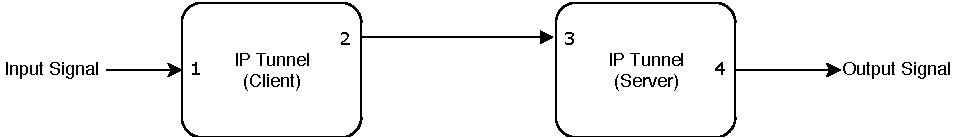
\includegraphics[width=1.0\textwidth]{./lib/ip_tunnel_ms_windows/figures/StructureTCPIP4.pdf}
	\label{IP Tunnel Block}\caption{IP Tunnel MS Windows block}
\end{figure}

\begin{figure}[h]
	\centering
	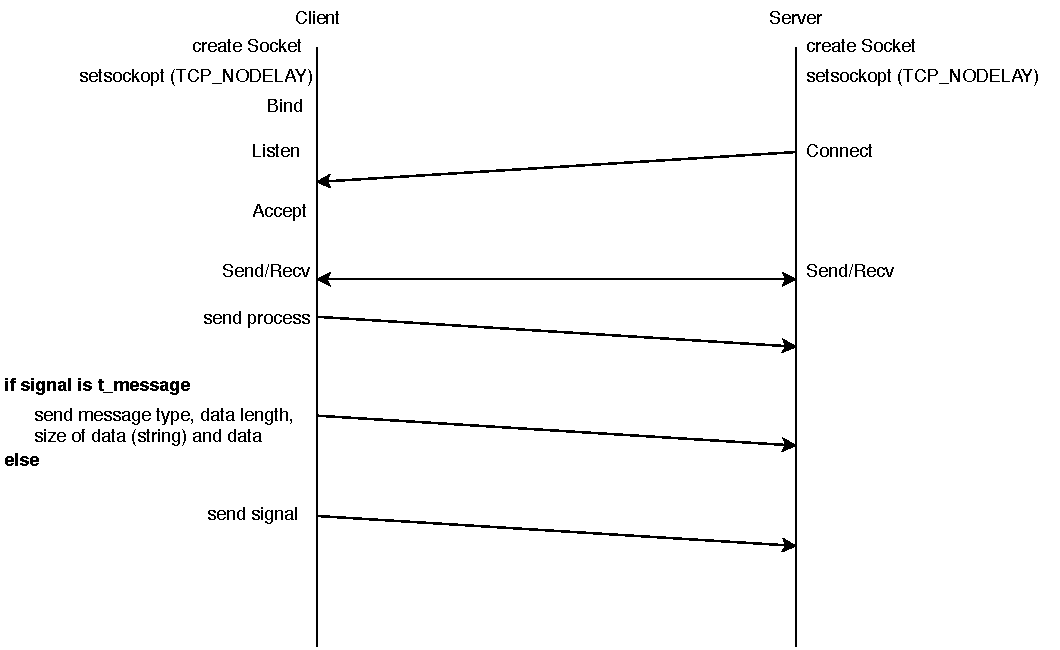
\includegraphics{./lib/ip_tunnel_ms_windows/figures/FluxogramIPTunnel.pdf}
	\label{IP Tunnel Block}\caption{IP Tunnel MS Windows block}
\end{figure}


\subsection*{Bandtwith testing}

This section was created to test the efficiency of the module in two environments: with Ethernet and with VPN.
In the folder "sdf" there are two other folders with the names "ip\_tunnel\_ms\_windows\_bandwith\_tx" for the client and "ip\_tunnel\_ms\_windows\_bandwith\_rx" for the server corresponding to the simulations between the two different computers.\par
The first experiment is between two computers in the same network with ethernet and bandwith of 100Mbps. Transmitting 8 million bits (1MB) in this setting, took about 148 seconds. 
\par

The second experiment is between two computers on different networks using VPN. The results are very similar as the module doesn't lose bandwith because of the VPN connection
